\documentclass[a4paper,
fontsize=11pt,
%headings=small,
oneside,
numbers=noperiodatend,
parskip=half-,
bibliography=totoc,
final
]{scrartcl}

\usepackage{synttree}
\usepackage{graphicx}
\setkeys{Gin}{width=.4\textwidth} %default pics size

\graphicspath{{./plots/}}
\usepackage[ngerman]{babel}
\usepackage[T1]{fontenc}
%\usepackage{amsmath}
\usepackage[utf8x]{inputenc}
\usepackage [hyphens]{url}
\usepackage{booktabs} 
\usepackage[left=2.4cm,right=2.4cm,top=2.3cm,bottom=2cm,includeheadfoot]{geometry}
\usepackage{eurosym}
\usepackage{multirow}
\usepackage[ngerman]{varioref}
\setcapindent{1em}
\renewcommand{\labelitemi}{--}
\usepackage{paralist}
\usepackage{pdfpages}
\usepackage{lscape}
\usepackage{float}
\usepackage{acronym}
\usepackage{eurosym}
\usepackage[babel]{csquotes}
\usepackage{longtable,lscape}
\usepackage{mathpazo}
\usepackage[normalem]{ulem} %emphasize weiterhin kursiv
\usepackage[flushmargin,ragged]{footmisc} % left align footnote
\usepackage{ccicons} 

%%%% fancy LIBREAS URL color 
\usepackage{xcolor}
\definecolor{libreas}{RGB}{112,0,0}

\usepackage{listings}

\urlstyle{same}  % don't use monospace font for urls

\usepackage[fleqn]{amsmath}

%adjust fontsize for part

\usepackage{sectsty}
\partfont{\large}

%Das BibTeX-Zeichen mit \BibTeX setzen:
\def\symbol#1{\char #1\relax}
\def\bsl{{\tt\symbol{'134}}}
\def\BibTeX{{\rm B\kern-.05em{\sc i\kern-.025em b}\kern-.08em
    T\kern-.1667em\lower.7ex\hbox{E}\kern-.125emX}}

\usepackage{fancyhdr}
\fancyhf{}
\pagestyle{fancyplain}
\fancyhead[R]{\thepage}

% make sure bookmarks are created eventough sections are not numbered!
% uncommend if sections are numbered (bookmarks created by default)
\makeatletter
\renewcommand\@seccntformat[1]{}
\makeatother


\usepackage{hyperxmp}
\usepackage[colorlinks, linkcolor=black,citecolor=black, urlcolor=libreas,
breaklinks= true,bookmarks=true,bookmarksopen=true]{hyperref}
%URLs hart brechen
\makeatletter 
\g@addto@macro\UrlBreaks{ 
  \do\a\do\b\do\c\do\d\do\e\do\f\do\g\do\h\do\i\do\j 
  \do\k\do\l\do\m\do\n\do\o\do\p\do\q\do\r\do\s\do\t 
  \do\u\do\v\do\w\do\x\do\y\do\z\do\&\do\1\do\2\do\3 
  \do\4\do\5\do\6\do\7\do\8\do\9\do\0} 
% \def\do@url@hyp{\do\-} 
\makeatother 

%meta
%meta

\fancyhead[L]{Redaktion LIBREAS \\ %author
LIBREAS. Library Ideas, 32 (2017). % journal, issue, volume.
\href{http://nbn-resolving.de/}
{}} % urn 
% recommended use
%\href{http://nbn-resolving.de/}{\color{black}{urn:nbn:de...}}
\fancyhead[R]{\thepage} %page number
\fancyfoot[L] {\ccLogo \ccAttribution\ \href{https://creativecommons.org/licenses/by/3.0/}{\color{black}Creative Commons BY 3.0}}  %licence
\fancyfoot[R] {ISSN: 1860-7950}

\title{\LARGE{Editorial \#32: Wirkung von Open Access}} % title
\author{Redaktion LIBREAS} % author

\setcounter{page}{1}

\hypersetup{%
      pdftitle={Editorial \#32: Wirkung von Open Access},
      pdfauthor={Redaktion LIBREAS},
      pdfcopyright={CC BY 3.0 Unported},
      pdfsubject={LIBREAS. Library Ideas, 32 (2017).},
      pdfkeywords={Open Access},
      pdflicenseurl={https://creativecommons.org/licenses/by/3.0/},
      pdfcontacturl={http://libreas.eu},
      baseurl={http://libreas.eu},
      pdflang={de},
      pdfmetalang={de}
     }



\date{}
\begin{document}

\maketitle
\thispagestyle{fancyplain} 

%abstracts

%body
Blättert oder vielmehr browst man durch das Archiv der nunmehr 31
LIBREAS. Library Ideas-Ausgaben der vergangenen zwölf Jahre, dann fällt
-- nicht überraschend -- auf, dass das Thema Open Access in seinen
unterschiedlichsten Facetten, von (disziplinären) Publikationskultur(en)
und -ideologien bis hin zu (bibliothekarischen)
Infrastrukturdienstleistungen in nicht wenigen Beiträgen bereits
beleuchtet wurde. Am auffälligsten und intensivsten geschah dies in den
beiden Ausgaben von 2009 mit dem Schwerpunktthema \enquote{Open Access
in den Geisteswissenschaften}. So finden sich in der Ausgabe \#15 (2009)
die rückblickend exemplarisch wirkenden kontroversen Positionen von Uwe
Jochum und Joachim Eberhardt zu Open Access.\footnote{Vgl. Uwe Jochum,
  "Der Souverän. ". LIBREAS. Library Ideas, 15 (2009).
  \url{http://libreas.eu/ausgabe15/texte/006.htm} und Joachim Eberhardt,
  "Wiederholung erzeugt keine Wahrheit. Jochum schreibt immer noch gegen
  Open Access. ". LIBREAS. Library Ideas, 15 (2009).
  \url{http://libreas.eu/ausgabe15/texte/007.htm}.} Die prinzipielle
Debatte dauert bis heute an.

Neben immernoch stets definitorischen, aber auch zahlreichen praxisnahen
Betrachtungen in der einschlägigen Fachliteratur, spiegelt sie sich auch
öffentlichkeitswirksam in den Zeitungs-\footnote{exemplarisch: Roland
  Reuss: Staatsautoritarismus, groß geschrieben. In: FAZ.net,
  30.09.2016,
  http://www.faz.net/aktuell/feuilleton/forschung-und-lehre/open-access-strategie-staatsautoritarismus-gross-geschrieben-14454601.html}
und nun auch Github-Feuilletons wieder. Oder sie manifestiert sich in
einer Initiative \enquote{Publikationsfreiheit für bessere
Bildung}\footnote{Vgl. \url{https://www.publikationsfreiheit.de/}.},
deren Ton stark an den Heidelberger Appell\footnote{Vgl. zum Überblick
  und weiterführender Literatur:
  \url{https://de.wikipedia.org/wiki/Heidelberger_Appell}.} vor acht
Jahren erinnert -- fraglos einem Höhepunkt in der Geschichte der
OA-Debatte. Auch im LIBREAS.Blog waren und sind das Thema und der
dazugehörige Diskurs stets präsent.

Es kommt demnach nicht von ungefähr, dass sich die vorliegende Ausgabe
erneut schwerpunktmäßig dem freien Zugang zu wissenschaftlichen
Publikationen widmet.

In unserem Call for Papers fragten wir titelgebend: \enquote{Wirkt Open
Access? Oder: Wo ist die Utopie geblieben?} und skizzierten
zugespitzt-kursorisch die Entwicklung ausgehend von der sich in den
frühen Erklärungen von Budapest und Berlin manifestierenden Utopie von
Open Access als Lösung der Zeitschriftenkrise, der Entfaltung der
digitalen Kommunikationsmöglichkeiten und damit letztlich dem
uneingeschränkt (kosten-)freien, unwiderruflichen und weltweiten Zugang
zu Wissen für alle. Wir landeten bei einem Status Quo des Open Access
als attraktivem, dynamischem, ungebrochen politisch aufgeladenem
Geschäftsmodell beziehungsweise Geschäfts- und Servicefeld -- sowohl für
Verlage, als auch für Informationsinfrastruktureinrichtungen wie
Bibliotheken. Und nicht zuletzt als Diskursanker für die Förder- und
Wissenschaftspolitik.\footnote{Vgl. hierzu die DFG-Ausschreibung
  Open-Access-Transformationsverträge im Kontext der globalen
  OA2020-Initiative:
  \url{http://www.dfg.de/foerderung/info_wissenschaft/2017/info_wissenschaft_17_12/}.
  Konkret geschaffenes Instrument in Deutschland ist der nationale Open
  Access-Kontaktpunkt (\url{http://oa2020-de.org/}), der eng mit dem
  Projekten DEAL (\url{https://www.projekt-deal.de/}) und INTACT
  (\url{https://www.intact-project.org/}) kooperiert.}

Im Vergleich zu anderen Ausgaben der LIBREAS. Library Ideas führte in
der jetzigen Ausgabe \#32 die thematische Schwerpunktsetzung zu sehr
meinungsstarken Artikeln, die auch in ihren gesellschafts- und
wissenschaftspolitischen Ansätzen sehr breit aufgestellt sind. Wir, als
Redaktion, finden eine solche breite Debatte gut und würden sie uns
öfter wünschen. Gleichzeitig -- das sollte bei dieser Breite
selbstverständlich sein -- sind wir inhaltlich nicht notwendig mit jedem
Artikel einverstanden.

\begin{figure}
\centering
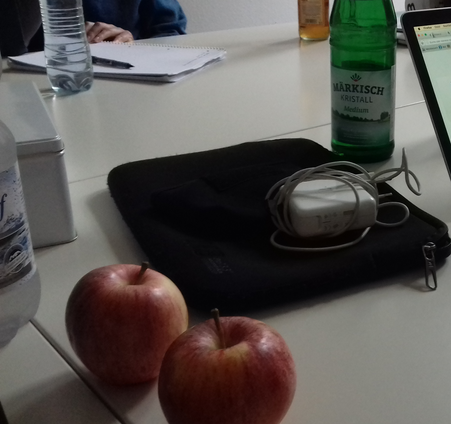
\includegraphics{editorial.png}
\caption{Redaktionsorte XI: Berlin, 22.10.2017}
\end{figure}

\hypertarget{zu-einigen-beitruxe4gen}{%
\subsubsection{Zu einigen Beiträgen}\label{zu-einigen-beitruxe4gen}}

In unserem Interview mit einem Aktiven aus dem Umfeld der
Sci-Hub-Schattenbibliothek wird deutlich, dass diese Form der
Datensammlung nicht etwa nur ein Ergebnis illegaler Zugriffe oder von
Hackerangriffen ist, sondern auch das Resultat einer freiwilligen
Kollaboration diverser Akteure. Unter anderem sind auch
wissenschaftliche Bibliothekar/innen beteiligt. Gerade deshalb steuert
die von den betroffenen Wissenschaftsverlagen versuchte Kriminalisierung
im Deutungskampf ins Leere, denn auch die Lesart des, wenn man so will,
zivilen Ungehorsams wird möglich. Wenn nämlich Wissenschaftler/innen und
Bibliothekar/innen auf diesen Zug einer Selbstversorgung aufspringen,
ist dies ein deutliches Signal und als Indikator für die Stimmung in
dieser Gruppe beziehungsweise den entsprechenden Institutionen
anzusehen. Das Engagement der Bibliothekar/innen zeigt, dass zumindest
einige unter ihnen nicht mehr gewillt sind, ihre Institution umstandslos
einer Marktlogik auszuliefern, auch wenn das so vorgesehen scheint.
Bibliotheken, die nur noch als Lizenzverwalter praktisch
oligopolistischer Wissenschaftsverlage fungieren und alle
Preiserhöhungen oder neuen Abnahmemodelle (Zwangsabnahme von gedruckten
Ausgaben bei Bestellung von digitalen Angebote et cetera) tolerieren
müssen, arbeiten systematisch gegen sich -- wenn nicht als
stabilisierende Faktoren dieses Systems sogar gegen ihren eigenen
Auftrag. Die stillschweigende Kooperation einzelner
Bibliotheksangestellter mit Sci-Hub muss als partielle Auflösung dieses
Widersinns angesehenen werden und stellt sozusagen einen Widerstand aus
dem herrschenden System heraus dar. Es ist rückhaltlos zu begrüßen (und
vielen anderen Institutionen zu wünschen), dass sich Angestellte vom
Status willenloser Erfüllungsgehilfen emanzipieren, wenn Politik
fahrlässig wird oder gar absichtlich Institutionen aufgeklärter
Umgangsformen bedroht. Ob Sci-Hub der richtige Kanal ist und welche
Interessen hier bedient werden, soll an dieser Stelle offen bleiben. In
jedem Fall scheint die Existenz dieser doch im Stillen weithin
akzeptierten Streaming- und Download-Vermittlung ein wirksames Mittel,
um an einer anderen Stelle mit deutlich mehr Gewicht in die
Verhandlungen mit den großen Wissenschaftsverlagen zu treten.

Gern würden wir von unseren Leser/innen erfahren, ob diese Lesart
geteilt wird. Um das Maß der auch öffentlich zu demonstrierenden
Solidarität\footnote{Vgl. hierzu Dušan Barok, Josephine Berry, Bodó
  Balázs et al.: In solidarity with Library Genesis and Sci-Hub. In:
  \url{http://custodians.online/}, 30.11.2015 {[}Zugriff am
  16.12.2017{]}.} zu erwägen, die nötig werden könnte, muss betont
werden, dass in den genannten Fällen Lohnabhängige ohne individuelle
Vorteile ihre Erwerbsgrundlage aufs Spiel setzen, um dem Ideal der
freien Zirkulation von Wissen ein wenig mehr Genüge zu tun. Wem das als
\enquote{Wissenskommunismus} erscheint, der sollte erwägen, dass genau
das schon lange als eine der wesentlichen Grundlagen von moderner
Wissenschaft angesehen wird, zu deren Sicherung (wissenschaftliche)
Bibliotheken bekanntlich genuin beitragen sollen.

Die Ausgabe enthält diesmal drei Interviews. Neben dem schon genannten,
zwei weitere mit Akteuren aus der Open Access-Community, die sich
reichlich kritisch zu den Entwicklungen der letzten Jahre äußern. Die
LIBREAS. Library Ideas ist neben wissenschaftlichen Artikeln und Essays
immer offen für unterschiedliche Textformate. Die Interviews können
(neben ihrem Inhalt) als Beispiel dafür gelten, was möglich ist. Wir als
Redaktion hoffen, in folgenden Ausgaben mehr solcher anderer
Beitragsformen zu sehen.\footnote{Dabei ist die Breite der möglichen
  Beiträge so weit, wie die stilistischen und technischen Möglichkeiten.
  Freie Formate, Bildstrecken, Berichte und Kommentare sind ebenso gerne
  gesehen, wie empirischen Beiträge(beispielsweise dynamischer Formate
  wie R Markdown, so dass sich Analysen technisch nachvollziehen
  lassen). Mittels GitHub, über das LIBREAS. Library Ideas quelloffen
  gehostet wird, ist auch die gemeinsame Veröffentlichung von
  dynamischen Abbildungen, Daten oder Skripten möglich. Wir bewegen uns
  in der Bibliotheks- und Informationswissenschaft in einem sehr weitem
  Feld zwischen hoher Praxisorientierung (\enquote{meine Bibliothek}),
  hoher Technik- und Innovationsorientierung (Data Science) und
  Orientierung an sehr unterschiedlichen Wissenschaftsfeldern
  (Soziologie, Informatik, Kultur- und Medienwissenschaft, Philosophie
  und so weiter). Dies soll sich auch in der LIBREAS. Library Ideas
  widerspiegeln.}

Andere Artikel zeigen die schon angesprochene Breite der Meinungen,
Initiativen und Erfahrungen im Bereich Open Access auf. Das Thema lässt
sich schon lange nicht mehr auf einige, wenige gemeinsame Punkte
reduzieren. Stattdessen hat sich die Bewegung ausdifferenziert,
professionalisiert (beispielsweise in Open Access Büros) und teilweise
auch Enttäuschungen hervorgebracht. Hervorzuheben sind die Texte von
Nikolaus Hamann, Anita Cymborska und Frank Havemann, die aus
unterschiedlichen Perspektiven nach Grenzen der heutigen Praxis von Open
Access und nach bislang vergebenen Potentialen fragen.

\hypertarget{neue-kolumne}{%
\subsubsection{Neue Kolumne}\label{neue-kolumne}}

In dieser Ausgabe erscheint zum ersten Mal die Kolumne \enquote{Das
liest die LIBREAS}, eine Medienschau in der Bibliotheks- und
Informationswissenschaft sowie des Bibliothekswesens. Die Grundideen der
Kolumne haben wir in ihr selber dargestellt. Ihr Ziel ist, einen kurzen
Überblick zu Publikationen (in verschiedenen Formaten, von Monographien
und Artikel über Social Media bis hin zu Konferenzen) zu geben, die
jeweils in der letzten Zeit im genannten Feld erschienen sind oder für
das Feld Relevanz haben.\footnote{Vgl.
  \url{https://libreas.wordpress.com/2017/11/08/das-liest-die-libreas-zu-einer-neuen-kolumne-eine-einladung-zur-mitarbeit/}}
Sie ist gedacht als ein lebendiger Text, zu dem alle Leser/innen gerne
beitragen können. Zudem unterstützt sie den Vereinszweck von LIBREAS.
Verein\footnote{Vgl. \url{http://www.libreas-verein.eu/}}, in welchem
weiterhin Mitglieder/innen sehr willkommen sind.

Ihre / eure Redaktion LIBREAS. Library Ideas

(Berlin, Chur, Dresden, Hannover, München)

%autor

\end{document}
